\documentclass[11pt,a4paper]{article}
\usepackage{hw}
\usepackage{subcaption}

\graphicspath{ {.} }
\setlength\parindent{0pt}

\begin{document}
\qtitle{Ex1}
To compute the angle between image pairs, cosine similarity is first computed as $sim=cos(\theta)=\cfrac{u\cdot v}{\|u\| \|v\|}$, then the angle is $\theta=arccos(sim)$. 

\begin{lstlisting}
import numpy as np
import os 
import glob
import cv2
import math

# exercise 1
root_dir = "BIOE580_hw01_data"
image_dir = "hw01_ex01_fastMRI-T1-brain-slices"
images = glob.glob(os.path.join(root_dir, image_dir+"/*.png"))

print(",".join(images)+"\n")
for img_a in images:
    frame_a = cv2.imread(img_a)
    # normalize image 
    frame_a = frame_a / 255
    print("{}:".format(img_a), end="")
    vector_a = np.ravel(frame_a)
    for img_b in images:
        frame_b = cv2.imread(img_b)
        frame_b = frame_b / 255
        vector_b = np.ravel(frame_b)
        # compute cosine similarity
        cos_sim = np.inner(vector_a, vector_b) / (np.linalg.norm(vector_a) * np.linalg.norm(vector_b))
        angle = np.arccos(cos_sim) / math.pi * 180
        print("{}/{},".format(cos_sim, angle), end="")
    print("\n")
\end{lstlisting}

The sample images are shown as Fig.~\ref{fig:ex1_samp} and the results are shown in the following table. We can observe that when two images are more visually similar, the angle between them is smaller, like image 62631 and 62626. 

\begin{figure}[!ht]
    \centering
    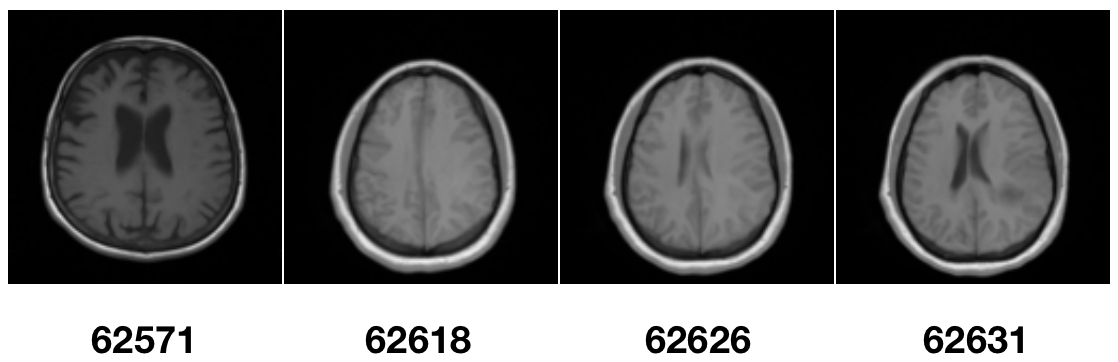
\includegraphics[width=0.8\linewidth]{ex1_samples.png}
    \caption{FastMRI examples}
    \label{fig:ex1_samp}
\end{figure}

\noindent\begin{minipage}{0.49\linewidth}
    \resizebox*{\textwidth}{!}{
    \begin{tabular}{c||c|c|c|c}
        \hline 
        Image ID & 62571 & 62631 & 62618 & 62626 \\
        \hline
        62571 & 1.00 & 0.76 & 0.77 & 0.76 \\
        62831 & 0.76 & 1.00 & 0.89 & 0.97 \\
        62618 & 0.77 & 0.89 & 1.00 & 0.96 \\
        62626 & 0.76 & 0.97 & 0.96 & 1.00 \\
        \hline
    \end{tabular}
    }
    \captionof{table}{Cosine similarity between image pairs.}
\end{minipage}
\hspace{0.1cm}
\begin{minipage}{0.49\linewidth}
    \resizebox*{\textwidth}{!}{
    \begin{tabular}{c||c|c|c|c}
        \hline 
        Image ID & 62571 & 62631 & 62618 & 62626 \\
        \hline
        62571 & 0.00 & 40.56 & 39.88 & 40.12 \\
        82831 & 40.56 & 0.00 & 27.55 & 14.99 \\
        62618 & 39.88 & 27.55 & 0.00 & 17.01 \\
        62626 & 40.12 & 14.99 & 17.01 & 0.00 \\
        \hline
    \end{tabular}
    }
    \captionof{table}{Angles between image pairs.}
\end{minipage}
\newpage

\qtitle{Ex2}
\textbf{a.} Operator H is a $16384\times 16384$-dimensional matrix which maps images from $16384$-dimensional space to objects in another $16384$-dimensional space. 

\textbf{b.} $\mathbf{H}:\mathbb{R}^{16384}\rightarrow \mathbb{R}^{16384}$

\textbf{c.} Because $H=H^T$, so $H$ is symmetric matrix. Also, $det(H)=0$, which means $H$ is singular matrix. H is not full rank and nullity $>$ 0. Therefore, $H$ has null space. 

\newpage
\qtitle{Ex3}
\textbf{a.} For $\mathbb{C}^2$, its standard basis vectors are $\{(1,0), (0,1)\}$.

$S_1\newvec{1&0\\0&1}=\mathcal{B}_1\rightarrow S_1=\mathcal{B}_1=\newvec{3&4\\4&-3}$

Similarly, the standard basis vectors of $\mathbf{C}^3$ are $\{(1,0,0), (0,1,0), (0,0,1)\}$. 

$S_2=\mathcal{B}_2=\newvec{1&2&2\\6&3&-6\\6&-6&3}$

\textbf{b.} $T\newvec{x\\y}=\newvec{x+yi\\x-yi\\2x}$. Easy to know: $T=\newvec{1&i\\1&-i\\2&0}$

$T_{new}=S_2^{-1}TS_1=\newvec{-0.6-44/15i&-0.8+2.2i\\
1.4+2.4i&28/15-1.8i\\0.4+16/15i&8/15-0.8i}$

\textbf{c.} $v=T_{new}u=\newvec{-2.8-56/15i\\3.2+64/15i\\1.2+1.6j}$

\textbf{d.} $u_e=S_1u=\newvec{3+4j\\4-3j}$

$v_e=S_2v=\newvec{6+8j\\0\\6+8j}$

We compute $T(u_e)=TS_1u=\newvec{6+8j\\0\\6+8j}=v_e$

\newpage 
\qtitle{Ex4}

According to Euler's equation, \\
$f(N)=\sum_{n=0}^{N-1}a_n(\cfrac{exp(in\pi x)-exp(-in\pi x)}{2i})+b_n(\cfrac{exp(in\pi x)+exp(-in\pi x)}{2})\\
=\sum_{n=0}^{N-1}\cfrac{b_n-ia_n}{2}exp(in\pi x)+\cfrac{b_n+ia_n}{2}exp(-in\pi x)$

$f(N)=\overline{f(N)}$. 
Since $u_n=\cfrac{1}{\sqrt{2}}exp(in\pi x)$, then $f(N)=\sum_{n=0}^{N-1}\cfrac{b_n-ia_n}{2}\sqrt{2}u_n+\cfrac{b_n+ia_n}{2}\sqrt{2}\overline{u_n}\\
=c_1u_n+c_2\overline{u_n}$

So f(N) is a linear combination of $u_n$ and its conjugate $\overline{u_n}$. So it seems that the dimension of $f(N)$ is 2 and $u_n$ could be a basis of f(N). 

For $u_n$, its inner product is:\\ 
$<u_n, u_n>=\bint{-1}{1}\cfrac{1}{\sqrt{2}}exp(-in\pi x)\cfrac{1}{\sqrt{2}}exp(in\pi x)dx=\bint{-1}{1}\cfrac{1}{2}dx=1$. \\
So $u_n$ is orthornormal basis. 

\newpage
\qtitle{5}
If $<\mathbf{f}, A\mathbf{g}>=<A\mathbf{f}, \mathbf{g}>$, then A is Hermitian.

For $A=iD$

$<A\mathbf{f}, \mathbf{g}> = \bint{-1}{1}\overline{Af}gdx=\bint{-1}{1}(-i\cfrac{d}{dx}\overline{f})gdx=-i\bint{-1}{1}gd\overline{f}$

$<\mathbf{f}, A\mathbf{g}>=\bint{-1}{1}\overline{f}i\cfrac{d}{dx}gdx=i\bint{-1}{1}\overline{f}dg$

$<A\mathbf{f}, \mathbf{g}>-<\mathbf{f}, A\mathbf{g}>=-i([g\overline{f}]_{-1}^1-\bint{-1}{1}\overline{f}dg)-i\bint{-1}{1}\overline{f}dg=-i[\overline{f}g]_{-1}^1=0$

$So $<A\mathbf{f}, \mathbf{g}>=<\mathbf{f}, A\mathbf{g}>$, A is hermitian. 

\newpage
\qtitle{Ex6}
Let $H=g(x',y')$, 

$H(af_1(x,y)+bf_2(x,y))=\bint{-\infty}{\infty}\bint{-\infty}{\infty}sinc(x'-x)sinc(y'-y)(af_1(x,y)+bf_2(x,y))dxdy\\
=a\bint{-\infty}{\infty}\bint{-\infty}{\infty}sinc(x'-x)sinc(y'-y)f_1(x,y)dxdy\\
+b\bint{-\infty}{\infty}\bint{-\infty}{\infty}sinc(x'-x)sinc(y'-y)f_2(x,y))dxdy\\
=aH(f_1(x,y))+bH(f_2(x,y))$

So $H=g(x',y')$ is a linear operator. 

Since sinc function is y-axis symmetric, $sinc(\theta)=\cfrac{sin(\theta)}{\theta}\rightarrow sinc(\theta)^\dagger=\cfrac{sin(-\theta)}{-\theta}=sinc(\theta)$

$H^\dagger=\bint{-\infty}{\infty}\bint{-\infty}{\infty}sinc(x'-x)^\dagger sinc(y'-y)^\dagger f(x,y)dxdy\\
=\bint{-\infty}{\infty}\bint{-\infty}{\infty}sinc(x'-x)sinc(y'-y)f(x,y)dxdy=H$. So it's Hermitian. 

Its domain should be $\mathbb{R}^2(-\infty, \infty)$ and its range may be $\mathbb{C}^1$ if sinc(x'-x) or sinc(y'-y) is complex. 


\newpage
\qtitle{Ex7}
\textbf{a.} 
\begin{figure}[!ht]
    \centering
    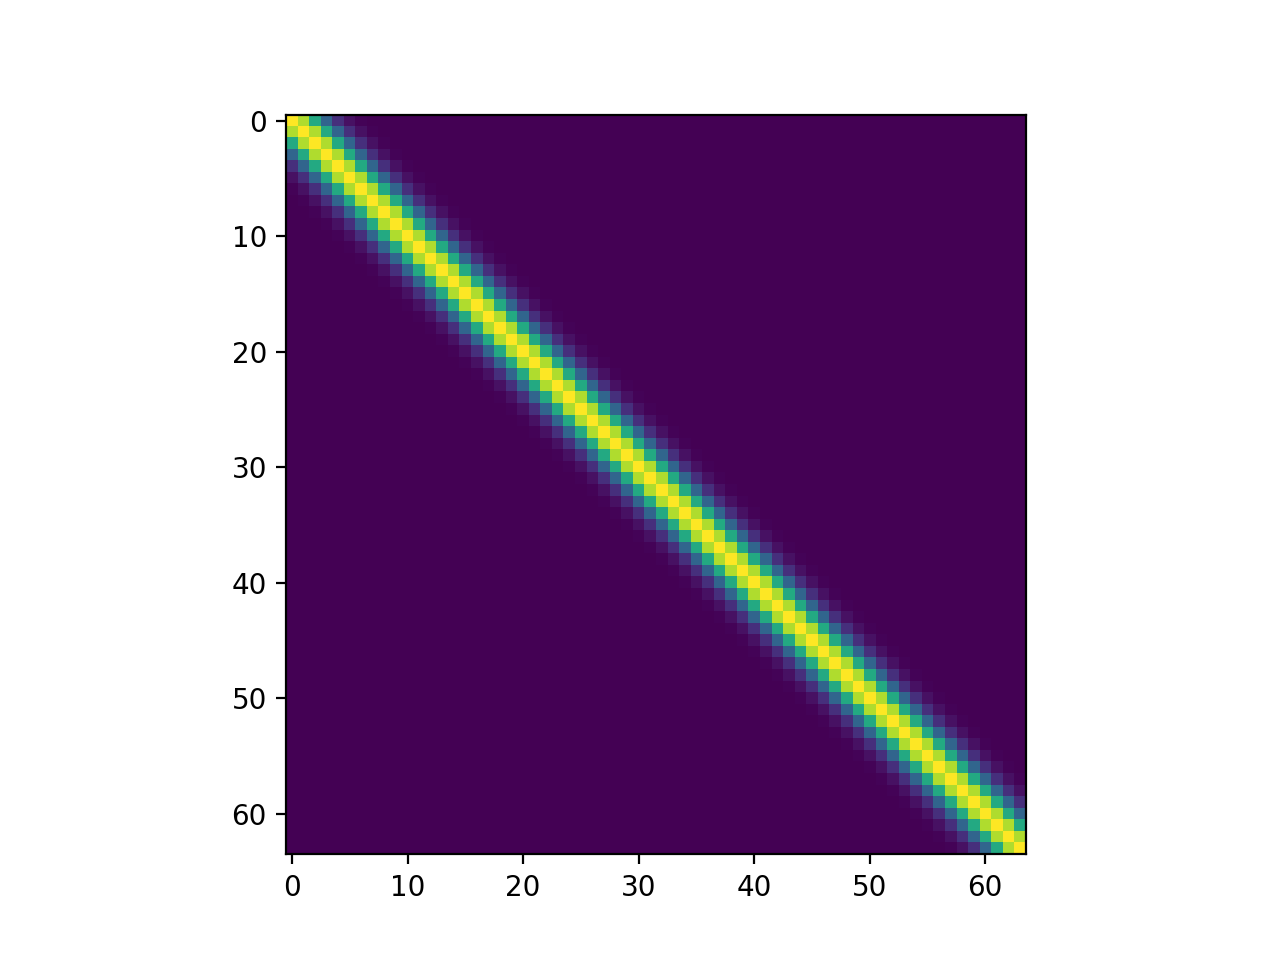
\includegraphics[width=0.6\linewidth]{ex7_heatmap.png}
    \caption{Heatmap of H when $\sigma=8$}
\end{figure}

\textbf{b.} $rank(H)=64$, so nullity(H)=64-64=0

\textbf{c.}
\begin{figure}[!ht]
    \centering
    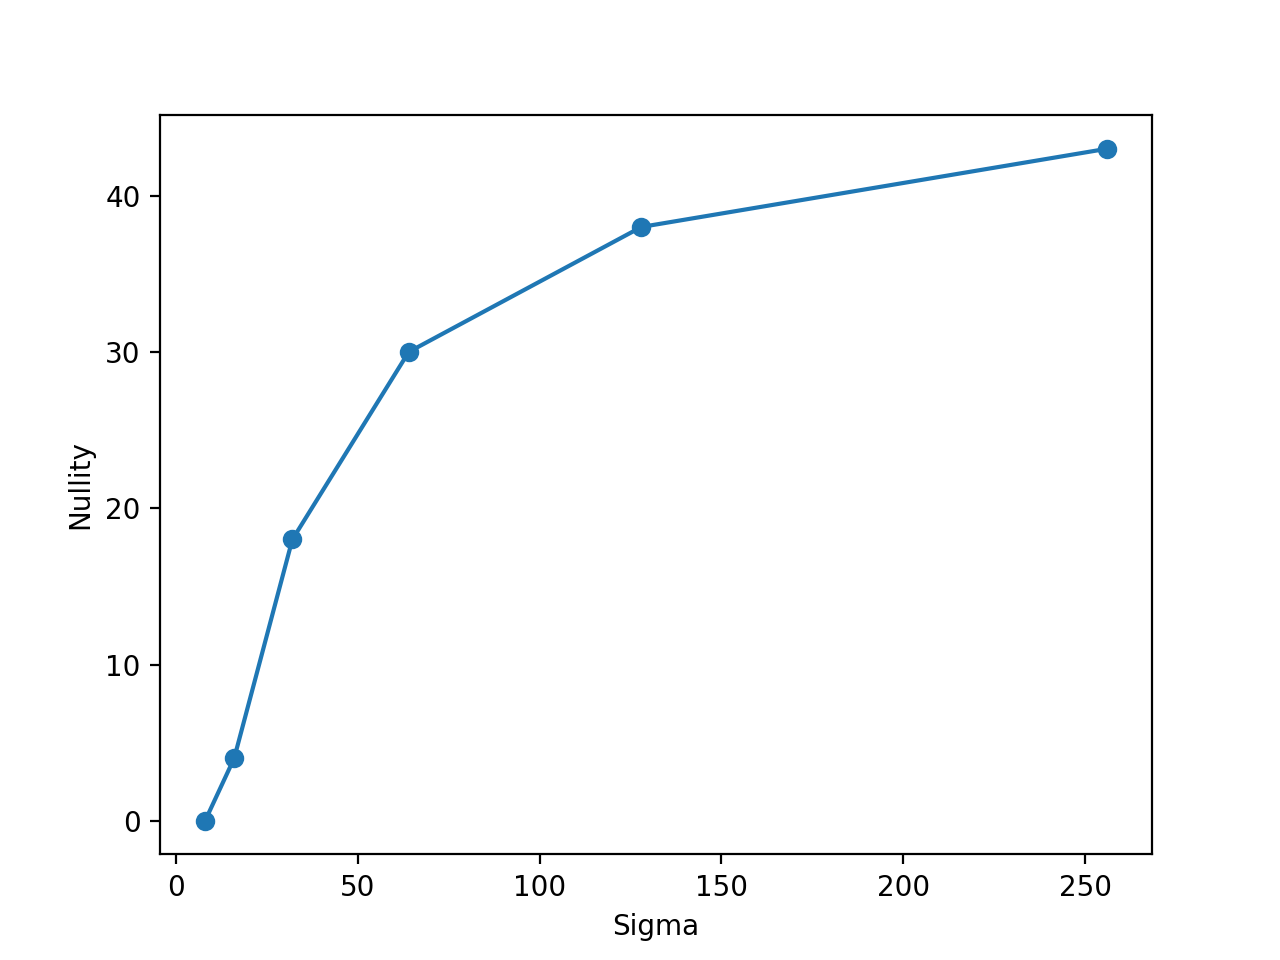
\includegraphics[width=0.6\linewidth]{ex7_nullity.png}
    \caption{Heatmap of H when $\sigma=8$}
\end{figure}

The nullity of operator H increases as $\sigma$ increases. When $\sigma$ increases sharply, the values which is closer to the diagonal line of H increases rapidly to 1. The column vectors become less orthogonal and more linearly dependent. So the rank of its column space decreases and the nullity increases.

\newpage
\qtitle{Ex8}
\textbf{a.}
To check whether $A$ is orthogonal, we compute $np.matmul(A, A.transpose())$ and the result shows that only diagonal values are close to 1 and the other values are trivial. So we can say $A$ is still orthogonal. 

\textbf{b.} 
Since $A$ is nearly-orthogonal, $P$ should be still nearly-orthogonal. Only diagonal values of $P$ are about 1, so $\sum_r\sum_cP_{r,c}=64$

\textbf{c.}
$P_{null}\perp P\rightarrow <P_{null}, P>=0$. Since $P$ is nearly-identity matrix, we could simply set $P_{null}=I-P$.

\textbf{d.}
\vspace{-1cm}
\begin{figure}[!ht]
    \centering
    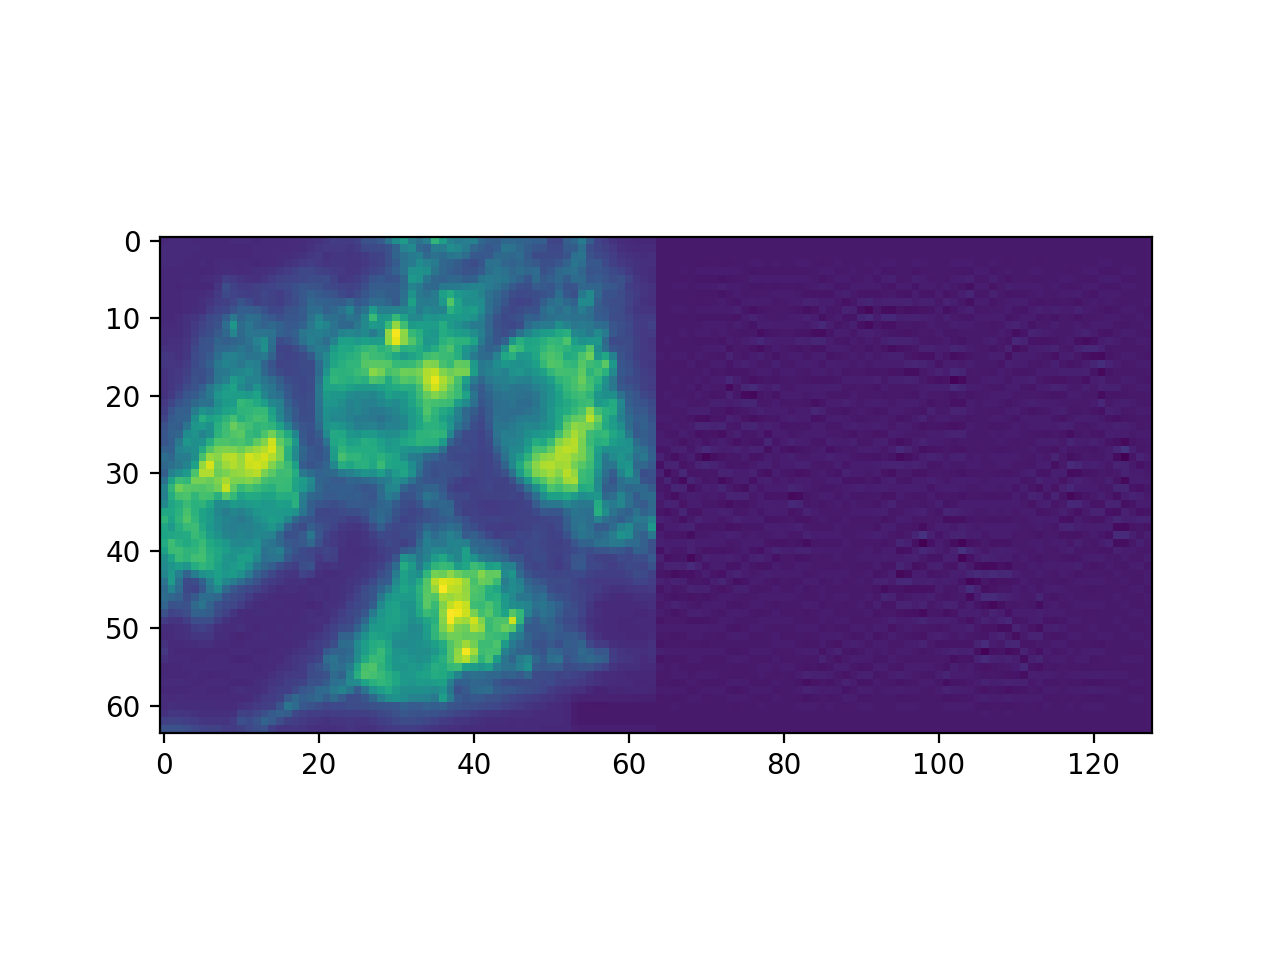
\includegraphics[width=0.6\linewidth]{ex8_forward.png}
    \vspace{-1cm}
    \caption{Projection result with $P$ and $P_{null}$}
\end{figure}

When applying $P$, the objective is projected into object space while preserving its major feature information. When applying $P_{null}$, the objective is projected into the null space, losing almost all information.

\textbf{e.} Use the code show in Ex1, the cosine similarity between the images is 0, which means the angle is $90^\circ$. The result is straightforward since $P_{null}\perp P\rightarrow P_{null}P=0$

\textbf{f.} Orthornormalization could make the basis orthogonal and normalized. On one hand, orthogonal matrix are computation efficiency which could keep the matrix sparse. On the other hand, normalization could keep matrix values within $[0,1]$ boundary, which is important to make space closed when employing operator for multiple times. Without normalization, the P could grow extremely big so that the computer cannot handle it. 
\end{document}
